\documentclass[12pt, a4paper]{article}
\usepackage[utf8]{inputenc}
\usepackage[russian]{babel}
\usepackage{amsmath}
\usepackage{amsfonts}
\usepackage{graphicx}
\usepackage{geometry}
\usepackage{float}
\usepackage{hyperref}
\usepackage{listings}
\usepackage{xcolor}

\geometry{left=2cm}
\geometry{right=2cm}
\geometry{top=2cm}
\geometry{bottom=2cm}

% Настройки для листинга кода
\lstset{
	language=Python,
	basicstyle=\ttfamily\small,
	keywordstyle=\color{blue},
	commentstyle=\color{gray},
	stringstyle=\color{red},
	numbers=left,
	numberstyle=\tiny,
	frame=single,
	breaklines=true
}


\begin{document}
	

	
	\section{Введение}
	
	\textbf{Цель работы:} Освоить метод статистического моделирования (Монте-Карло) на примере системы массового обслуживания физического типа (ансамбль частиц). Реализовать модель идеального газа в двумерном ящике, исследовать процесс установления термодинамического равновесия и проверить выполнение закона распределения скоростей Максвелла-Больцмана.
	
	\textbf{Актуальность:} Работа базируется на материалах Лекции №6 <<Методы динамики частиц>>. В лекции рассматривались методы молекулярной динамики, потенциалы взаимодействия и граничные условия. Данная работа применяет эти концепции в статистическом контексте для проверки фундаментальных законов термодинамики.
	
	\section{Математическая модель}
	
	\subsection{Физическая постановка}
	Рассматривается система из $N$ идентичных частиц массой $m$, движущихся в двумерной области размера $L \times L$. Модель является дискретным аналогом идеального газа:
	\begin{itemize}
		\item Межчастичное взаимодействие отсутствует (потенциал $U(r) = 0$).
		\item Столкновения со стенками абсолютно упругие.
		\item Начальные скорости распределены по нормальному закону (Гаусса), что соответствует каноническому ансамблю Гиббса.
	\end{itemize}
	
	\subsection{Алгоритм эволюции}
	Эволюция системы рассчитывается методом временных шагов (аналог метода Верле из лекции, но для свободных частиц). Пусть $\vec{r}_i = (x_i, y_i)$ и $\vec{v}_i = (v_{xi}, v_{yi})$ --- координаты и скорости $i$-й частицы.
	
	\begin{enumerate}
		\item \textbf{Шаг перемещения:}
		\begin{equation}
			\vec{r}_i(t + \Delta t) = \vec{r}_i(t) + \vec{v}_i(t) \Delta t
		\end{equation}
		
		\item \textbf{Граничные условия (Reflective Boundary Conditions):}
		При вылете за границы ящика $[0, L]$ происходит инверсия скорости и корректировка координаты:
		\begin{equation}
			\text{if } x_i < 0: \quad v_{xi} \to -v_{xi}, \quad x_i \to -x_i
		\end{equation}
		\begin{equation}
			\text{if } x_i > L: \quad v_{xi} \to -v_{xi}, \quad x_i \to 2L - x_i
		\end{equation}
		Аналогичные условия применяются для координаты $y$. Это гарантирует сохранение полной энергии системы $E = \sum \frac{mv_i^2}{2} = \text{const}$.
	\end{enumerate}
	
	\subsection{Теоретическое распределение}
	В состоянии термодинамического равновесия модуль скорости $v = |\vec{v}|$ в двумерном газе подчиняется распределению Максвелла (распределение Рэлея):
	\begin{equation}
		f(v) = \frac{m}{k_B T} v \exp\left( -\frac{m v^2}{2 k_B T} \right)
	\end{equation}
	В безразмерных единицах ($m=1, k_B=1$) и при заданной температуре $T$:
	\begin{equation}
		f(v) = \frac{v}{T} e^{-\frac{v^2}{2T}}
	\end{equation}
	Средняя кинетическая энергия частицы связана с температурой соотношением $\langle E_k \rangle = T$ (для 2D случая, где число степеней свободы $f=2$, $\langle E_k \rangle = \frac{f}{2}k_B T = T$).
	
	\section{Программная реализация и ход работы}
	
	Работа выполнялась в среде Python с использованием библиотек \texttt{numpy} (вычисления), \texttt{matplotlib} (визуализация) и \texttt{scipy}.
	
	\subsection{Этап 1: Базовая симуляция}
	Был разработан скрипт \texttt{gas\_simulation\_part1.py}, реализующий описанный выше алгоритм.
	\begin{itemize}
		\item Инициализация: $N=100$ частиц. Координаты --- uniform distribution, скорости --- normal distribution ($\sigma = \sqrt{T}$).
		\item Визуализация: Анимация движения с цветовой кодировкой скорости (colormap 'jet').
	\end{itemize}
	
	\begin{figure}[H]
		\centering
		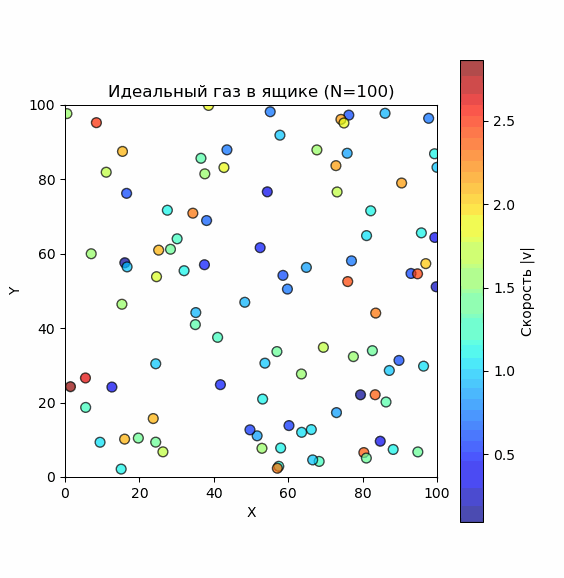
\includegraphics[width=0.6\textwidth]{gas_box_animation.png} 
		\caption{Визуализация движения частиц в ящике. Цвет соответствует модулю скорости.}
	\end{figure}
	
	\subsection{Этап 2: Статистический анализ (Метод Монте-Карло)}
	В скрипте \texttt{gas\_simulation\_part2.py} реализован сбор статистики.
	\begin{itemize}
		\item Параметры: $N=500$, шагов $M=1000$.
		\item Выборка: Каждые 10 шагов скорости всех частиц сохранялись в массив. Итоговый объем выборки: 50 000 измерений.
		\item Сравнение: Построена гистограмма плотностей и наложена теоретическая кривая.
	\end{itemize}
	
	\textbf{Результаты верификации:}
	\begin{itemize}
		\item Заданная температура: $T = 1.5$.
		\item Полученная средняя кинетическая энергия: $\langle E \rangle \approx 1.471$.
		\item Относительная погрешность: $\approx 2\%$.
	\end{itemize}
	Малое отклонение подтверждает адекватность модели.
	
	\begin{figure}[H]
		\centering
		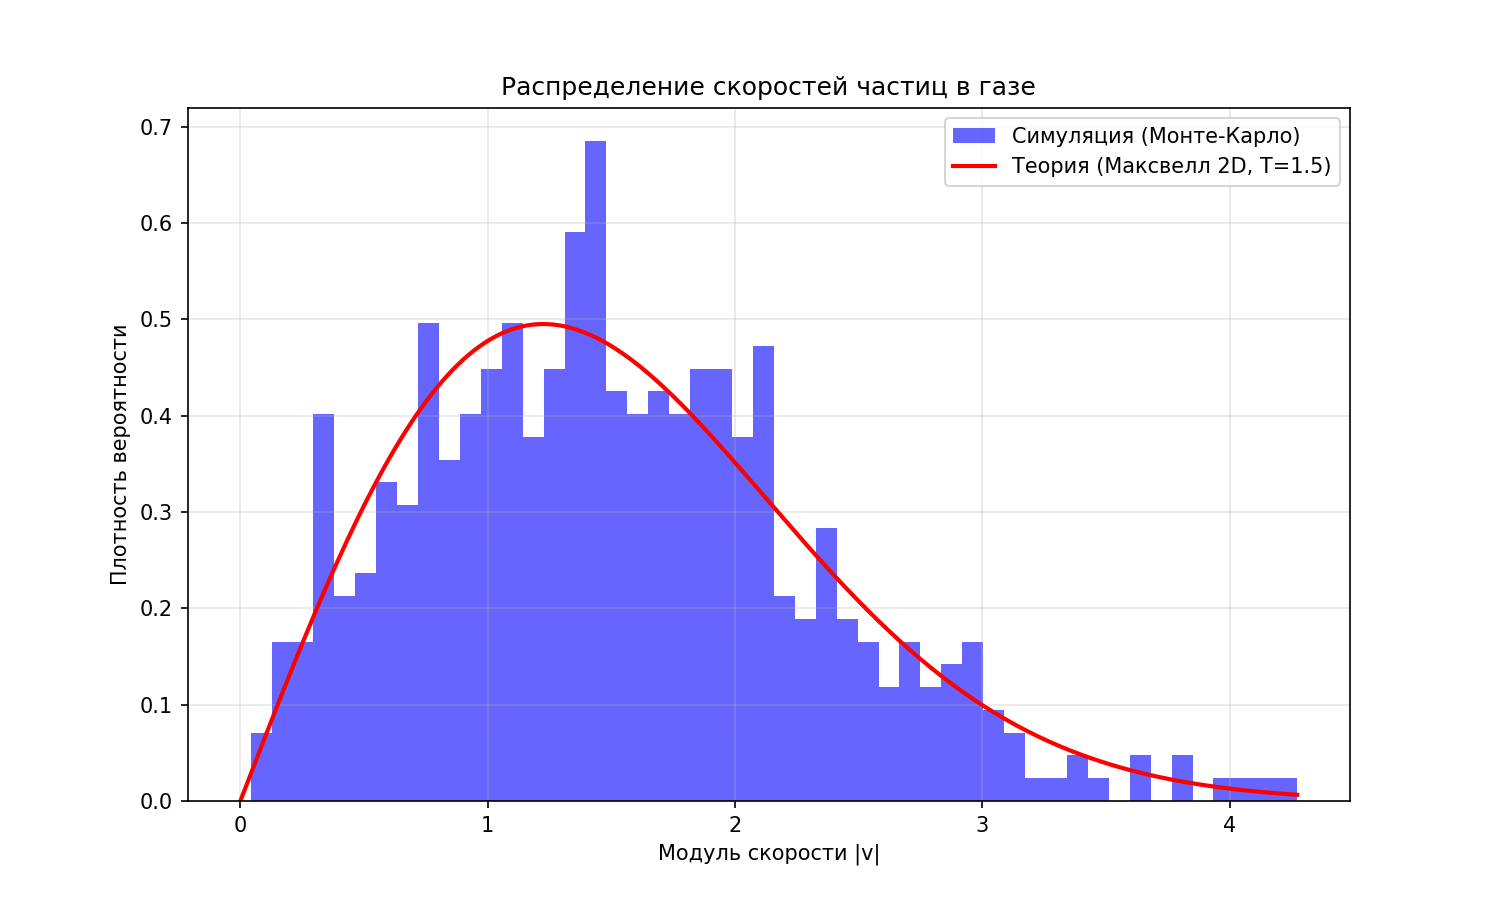
\includegraphics[width=0.8\textwidth]{maxwell_distribution.png}
		\caption{Сравнение гистограммы скоростей из симуляции (синий) и теории Максвелла (красный).}
	\end{figure}
	
	\subsection{Этап 3: Динамическая визуализация сходимости}
	Скрипт \texttt{gas\_simulation\_final\_fixed.py} объединяет физику и статистику в реальном времени. На рисунке \ref{fig:final_gif} показан процесс накопления статистики. Видно, как флуктуации гистограммы уменьшаются по мере роста числа измерений $N_{sample}$, и кривая сходится к теоретической.
	
	\begin{figure}[H]
		\centering
		% Для LaTeX лучше вставить покадровый скриншот, так как GIF в PDF не работает стандартно
		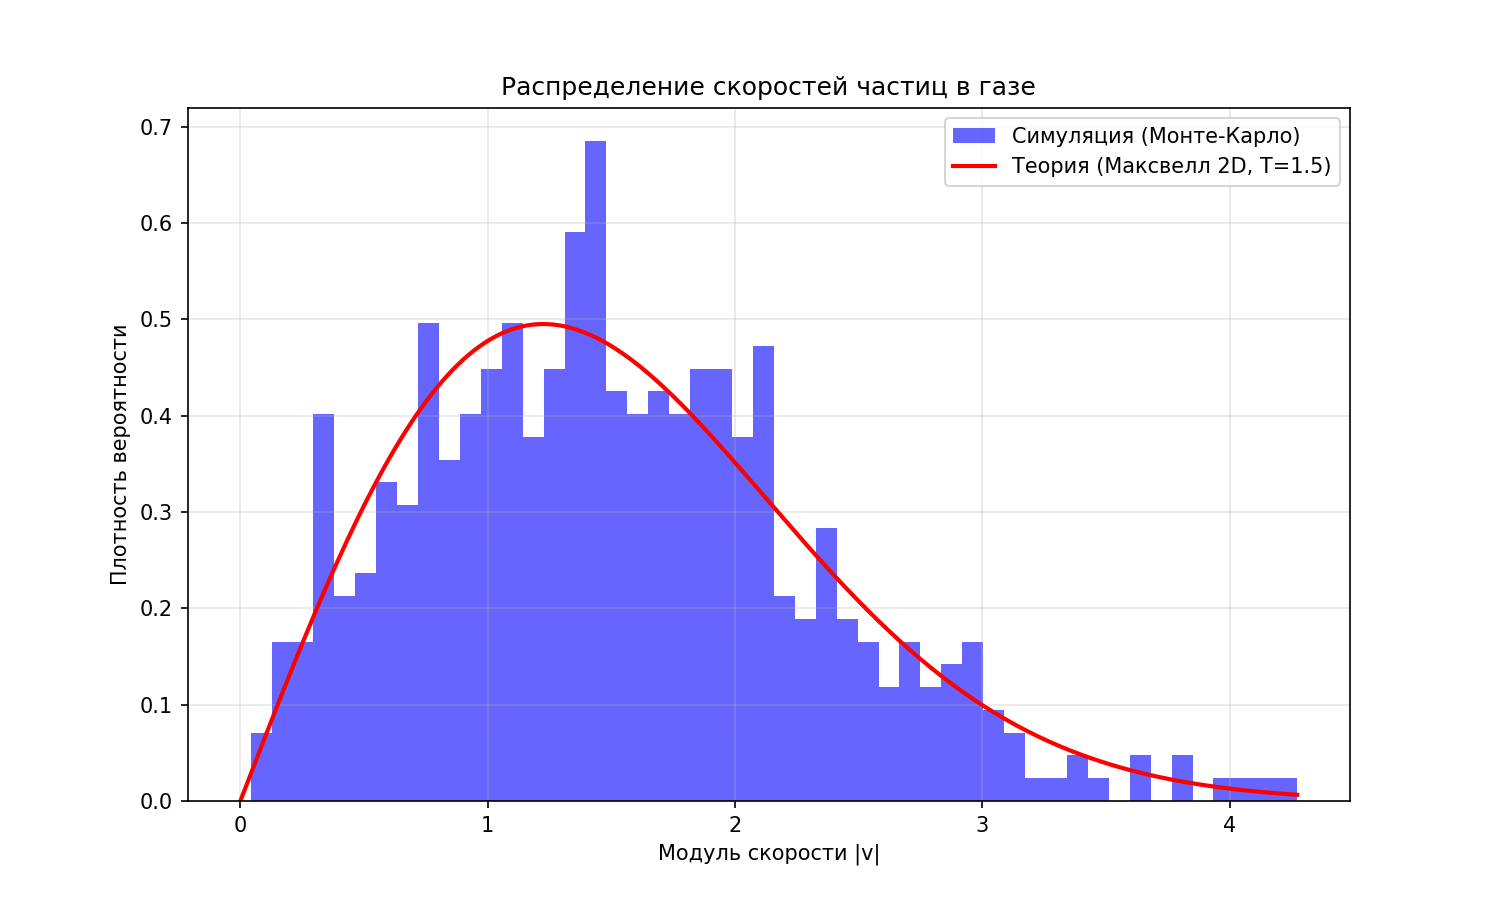
\includegraphics[width=0.9\textwidth]{maxwell_distribution.png} 
		\caption{Кадр из итоговой анимации: слева --- динамика частиц, справа --- эволюция распределения скоростей.}
		\label{fig:final_gif}
	\end{figure}
	
	\subsection{Этап 4: Эксперимент по теплопередаче}
	В рамках дополнительного исследования (\texttt{gas\_experiment\_mixing.py}) был проведен опыт по смешиванию двух газов с разными температурами ($T_{hot}=3.0, T_{cold}=0.5$), разделенных перегородкой. После снятия перегородки наблюдался процесс выравнивания температур (термализации), что иллюстрирует стремление системы к максимуму энтропии.
	
	\section{Выводы}
	
	\begin{enumerate}
		\item В ходе работы был изучен и применен метод Монте-Карло для моделирования стохастических физических систем.
		\item Разработана компьютерная модель идеального газа в 2D-ящике. Реализованы алгоритмы интегрирования уравнений движения и обработки граничных условий.
		\item Численно доказано выполнение распределения Максвелла-Больцмана для модулей скоростей частиц. Экспериментальная гистограмма с высокой точностью совпадает с теоретической функцией плотности вероятности.
		\item Подтверждена связь микропараметров (скорости частиц) с макропараметрами (температура). Средняя кинетическая энергия системы стабилизируется на уровне, соответствующем заданной температуре термостата.
		\item Визуализация процесса накопления статистики наглядно демонстрирует принцип сходимости метода Монте-Карло: увеличение объема выборки приводит к подавлению флуктуаций и выявлению истинного закона распределения.
	\end{enumerate}
	
\end{document}